%%%%%%%%%%%%%%%%%%%%%%%%%%%%%%%%%%%%%%%%%
% Short Sectioned Assignment
% LaTeX Template
% Version 1.0 (5/5/12)
%
% This template has been downloaded from:
% http://www.LaTeXTemplates.com
%
% Original author:
% Frits Wenneker (http://www.howtotex.com)
%
% License:
% CC BY-NC-SA 3.0 (http://creativecommons.org/licenses/by-nc-sa/3.0/)
%
%%%%%%%%%%%%%%%%%%%%%%%%%%%%%%%%%%%%%%%%%

%----------------------------------------------------------------------------------------
%	PACKAGES AND OTHER DOCUMENT CONFIGURATIONS
%----------------------------------------------------------------------------------------

\documentclass[letterpaper, fontsize=11pt]{scrartcl} % A4 paper and 11pt font size

\usepackage[T1]{fontenc} % Use 8-bit encoding that has 256 glyphs
\usepackage{fourier} % Use the Adobe Utopia font for the document - comment this line to return to the LaTeX default
\usepackage[english]{babel} % English language/hyphenation
\usepackage{amsmath,amsfonts,amsthm} % Math packages

\usepackage{lipsum} % Used for inserting dummy 'Lorem ipsum' text into the template

\usepackage[]{mcode} %MATLAB code

\usepackage{sectsty} % Allows customizing section commands
\allsectionsfont{\centering \normalfont\scshape} % Make all sections centered, the default font and small caps

\usepackage{fancyhdr} % Custom headers and footers
\usepackage{graphicx}
\pagestyle{fancyplain} % Makes all pages in the document conform to the custom headers and footers
\pagenumbering{arabic}
\fancyhead{} % No page header - if you want one, create it in the same way as the footers below
\fancyfoot[L]{\textit{CME 102 Winter '17-'18}} % Empty left footer
\fancyfoot[C]{\thepage} % Empty center footer
\fancyfoot[R]{Tim Anderson} % Page numbering for right footer
\renewcommand{\headrulewidth}{0pt} % Remove header underlines
\renewcommand{\footrulewidth}{0pt} % Remove footer underlines
\setlength{\headheight}{13.6pt} % Customize the height of the header

\numberwithin{equation}{section} % Number equations within sections (i.e. 1.1, 1.2, 2.1, 2.2 instead of 1, 2, 3, 4)
\numberwithin{figure}{section} % Number figures within sections (i.e. 1.1, 1.2, 2.1, 2.2 instead of 1, 2, 3, 4)
\numberwithin{table}{section} % Number tables within sections (i.e. 1.1, 1.2, 2.1, 2.2 instead of 1, 2, 3, 4)

\setlength\parindent{0pt} % Removes all indentation from paragraphs - comment this line for an assignment with lots of text
\begin{document}

%----------------------------------------------------------------------------------------
%	TITLE SECTION
%----------------------------------------------------------------------------------------

\newcommand{\horrule}[1]{\rule{\linewidth}{#1}} % Create horizontal rule command with 1 argument of height

%----------------------------------------------------------------------------------------
%	PROBLEM 1
%----------------------------------------------------------------------------------------

\section*{Week 2 Section Answers}
\par Solve the following problems. If initial conditions are given, solve for all constants of integration. It is okay to leave answers in implicit form or with unsolved integrals. 

\begin{enumerate}
\item \textbf{Linearity:} Show that the following ODEs are linear. If they are nonlinear, identify the nonlinear term and show that this term is nonlinear. \newline
\textbf{Solution} \newline Remember that when we are testing for linearity, we only examine the terms containing the dependent variable and its derivatives, not the independent variable. I.e. if we have an ODE for function $y(x)$, the linearity of the ODE is determined only by those terms containing $y$.
\begin{enumerate}
\item $sin(x)y''' + y = e^x$\newline
\textbf{Solution} Linear, because the terms $y'''$ and $y$ are both linear in $y$. Remember that a term or function $f(x)$ is linear in $x$ if
$$f(\alpha x + \beta y) = \alpha f(x) + \beta f(y)$$ This holds for both of these terms, and can be used to show the linearity or nonlinearity of the other terms for the rest of this problem. 
\item $y' + y^2 = tan(x)$\newline
\textbf{Solution} Nonlinear, because the term $y^2$ is not linear in $y$.
\item $y'' + 3sin(y) = 0$ \newline
\textbf{Solution} Nonlinear, because the term $sin(y)$ is not linear in $y$.
\item $y' + y = e^x$ \newline
\textbf{Solution} Linear, because the terms $y'$ and $y$ are linear in $y$.
\item $y' + y = e^y$ \newline
\textbf{Solution} Nonlinear, because the term $e^y$ is not linear in $y$.
\end{enumerate}

\item \textbf{Separation of Variables:} Solve the following using separation of variables. 
\begin{enumerate}
\item $y' = cot(y)$ \newline
\textbf{Solution} 
$$y' = \frac{dy}{dx} = cot(y)$$
$$\frac{dy}{cot(y)} = tan(y)dy = dx$$
Integrating both sides: $$ -ln(cos(y)) = x + c$$
$$y = cos^{-1}(e^{c-x})$$

\item $y' = y - y_0$
\textbf{Solution}
$$y' = y - y_0$$
$$\frac{dy}{y-y_0} = dx $$
$$ln|y-y_0| = x + c$$
$$y = Ce^x + y_0$$

\item $y' = 1 + e^{x} + e^{y} + e^{x + y}$ \newline
\textbf{Solution}
$$\frac{dy}{dx} = 1 + e^x + e^y + e^{x+y} = (1+e^x)(1+e^y)$$
$$\frac{dy}{1+e^y} = (1 + e^x)dx$$
$$\int \frac{dy}{1+e^y} = \int (1 + e^x)dx$$
$$\int \frac{e^{-y}dy}{e^{-y} + 1} = x + e^x + c$$
$$-ln(e^{-y} + 1) = x + e^x + c$$
$$e^{-y} + 1 = e^{c - x - e^x}$$
$$y = -ln(e^{c - x - e^x} - 1)$$

\end{enumerate}

\item \textbf{Direction fields, phase space, and stability:} For an ODE of the form $y' = f(x,y)$ (where $x$ and $y$ can also be vectors), we can find the fixed points through one of two ways. 
\begin{enumerate}
\item One method it to look at the direction field in $x$-$y$ space to find the fixed points and determine their stability. For the following figure, find the fixed points based on the direction field, and give their stability. \par
\begin{center}
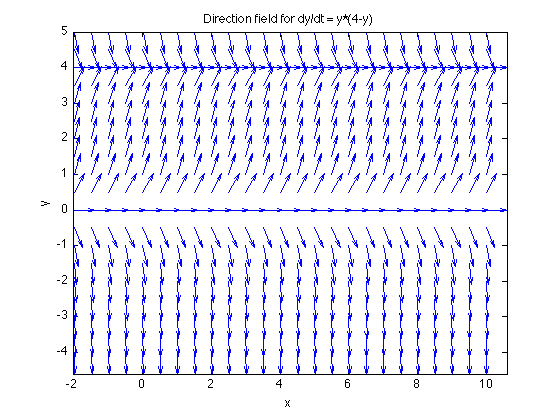
\includegraphics[width= 4in]{section2_1.png}
\end{center}
\textbf{Solution} \newline
Notice that the flows converge to the values $0$ and $4$. So, we see that $y = 0$ is an \textit{unstable} fixed point because the flows are stable at this point but diverge away (i.e. a slight perturbation will move the system away from $y = 0$). $y = 4$ is similarly a \textit{stable} fixed point or equilibrium because the direction field converges to $y = 4$, and a perturbation will bring you back to $y = 4$. \par
\item Another method is to examine function in what we call \textit{phase space}. This is where we plot the function value against its derivatives. In this case, we will plot the function in $y$-$y'$ space. For the following figure, find the fixed points by examine the function plotted against its derivative. Give the fixed points and their stability. \textit{Hint:} recall that a fixed point is where $y' = 0$. \newline
\begin{center}
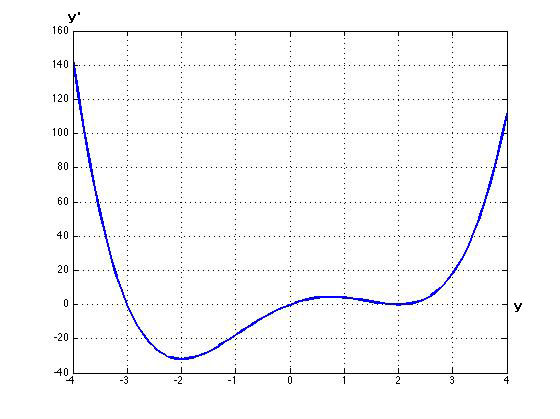
\includegraphics[width= 4in]{section2_2.jpg}
\end{center} \par
\textbf{Solution} \newline
Recall that an equilibrium is where $y' = 0$. This is simply the zeros of the phase-space plot! This function has $y'=0$ at $y=-3$, $y = 0$, and $y=2$. We can evaluate the stability of the fixed point from the phase space plot also. A rule of thumb for this is: if the sign of the derivative is opposite the sign of the change in the function, that direction is stable, and if the signs are the same it is unstable. So, $y=-3$ is a stable equilibrium since if you move to the left, the derivative is positive and moves the function back to the right, and if you move to the right the derivative is negative and returns you to the equilibrium. By the same rule, $y = 0$ is an unstable equilibrium. Lastly, notice that one side of $y=2$ is stable and one is unstable. In this case, $y=2$ is what we call a \textit{semi-stable} equilibrium. 
\end{enumerate}
Phase space is a very powerful tool in the field of dynamical systems. In fact, it was by analyzing phase space that mathematicians discovered  phenomena such as attractors and limit cycles, which ultimately kicked off the exciting field of chaos theory.

\item \textbf{MATLAB:} Write a \textit{small} piece of MATLAB code for each of the following functions. 
\begin{enumerate}
\item Output every multiple of 5 from 0 to 100. \textit{Hint:} the remainder of number $a$ after division by $b$ is given by mod($a$,$b$). \newline
\textbf{Solution}
\begin{lstlisting} 
for i = 0:100
	if mod(i,5) == 0
		i
	end	
end
\end{lstlisting}

\item Plot the functions $f_1(y) = y^2 + 1$ and $f_2(y) = y + 1$ over the domain $y \in [0,5]$ on the same graph in different colors with line thickness at 2pt. Pick a small enough increment in $y$ that the resolution of $f_1$ and $f_2$ is good. \newline
\textbf{Solution}
\begin{lstlisting} 
x = 0:0.01:5;
f1 = x.^2 + 1; 
f2 = x + 1;
plot(x,f1,x,f2,'LineWidth',2)
\end{lstlisting}
\item Write a function that will take two numbers as arguments and output their sum plus five i.e. $f(a,b) = a + b + 5$.  \newline
\textbf{Solution}
\begin{lstlisting} 
function c = myfunction(a,b)
	c = a + b + 5;
end
\end{lstlisting}

\end{enumerate}

\end{enumerate}

%----------------------------------------------------------------------------------------

\end{document}